\section*{Ejercicio \#1}
La figura \ref{fig:generador} presenta un código en lenguaje \verb!C++! para generar vectores de números aleatorios. Se empiezan con tamaños de diez mil en diez mil hasta llegar a dos cientos mil, generado así veinte muestras.
\begin{figure}[H]
  \centering
  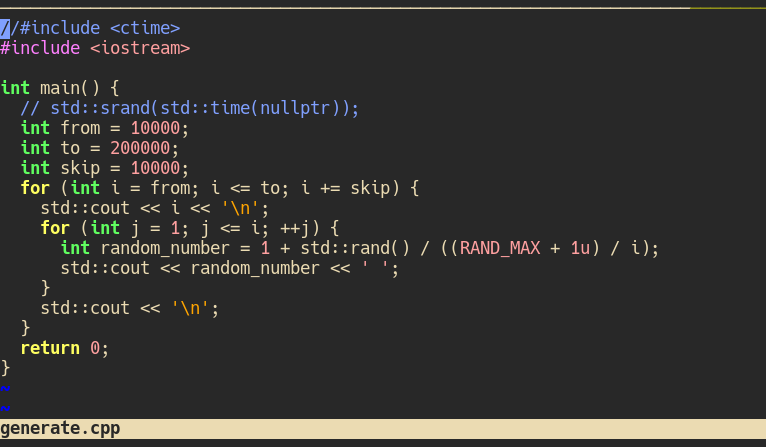
\includegraphics[width=0.8\textwidth]{generador}
  \caption{Generador de números aleatorios.}
  \label{fig:generador}
\end{figure}

El resultado se puede guardar en un archivo de texto, para pasarlo como entrada a ejecutables. Esto con el fin de poder analizar sobre el mismo conjunto de datos la \textit{performance} de los diferentes algoritmos de ordenamiento.

El código correspondiente se encuentra en la carpeta \href{https://github.com/syordya/CSUNSA-EDA/tree/master/Practica01/utils}{utils} del repositorio de la Práctica01.

\iffalse
% ---- Para poner dos imágenes (una a lado de otra) ----
Como se muestra en la figuras \ref{fig:act-1_a} y \ref{fig:act-1_b}.
\begin{figure}[H]
\centering
\begin{minipage}{0.45\textwidth}
  \centering
  \includegraphics[width=0.9\textwidth]{act-1_a}
  \caption{Envío de \textit{ICMP ECHO REQUEST} de PC0 a PC1, PC2 y PC3.}
  \label{fig:act-1_a}
\end{minipage}\hfill
\begin{minipage}{0.45\textwidth}
  \centering
  \includegraphics[width=0.9\textwidth]{act-1_b}
  \caption{Respuesta de PC1, PC2 y PC3. Tabla ARP de PC0.}
  \label{fig:act-1_b}
\end{minipage}
\end{figure}
% ---- Para colocar una imagen ----
Como se muestra en la figura \ref{fig:act-3}
\begin{figure}[H]
  \centering
  \includegraphics[width=0.8\textwidth]{act-3}
  \caption{Tabla de subneteo para la red 192.168.100.0.}
  \label{fig:act-3}
\end{figure}
\fi